\documentclass[11pt,letterpaper]{article}
\usepackage[margin=1in]{geometry}
\usepackage[T1]{fontenc}
\usepackage{newtxtext,newtxmath}
\usepackage{graphicx,booktabs,xcolor,amsmath,microtype,tikz,enumitem,caption,array}
\usepackage[hidelinks]{hyperref}
\usetikzlibrary{positioning,fit,arrows.meta,calc,backgrounds,decorations.pathreplacing}
\captionsetup{font=small,labelfont=bf}
\setlist{itemsep=2pt,topsep=4pt,leftmargin=1.4em}
\setlength{\parskip}{4pt}
\definecolor{cblue}{HTML}{2a78d6}
\definecolor{corange}{HTML}{eb6834}
\definecolor{caqua}{HTML}{1baf7a}
\definecolor{cpurple}{HTML}{8c5bd6}
\definecolor{cgray}{HTML}{8a8984}
\newcommand{\code}[1]{\texttt{\small #1}}
\newcommand{\shape}[1]{\texttt{\footnotesize[#1]}}
\tikzset{
  arr/.style={-{Stealth[length=5pt]},draw=black!60,thick},
  box/.style={draw=#1!80!black,fill=#1!10,rounded corners=2pt,inner sep=4pt,align=center},
  box/.default=cgray,
}

\title{\Large\bfseries How PickNet Works\\[2pt]\large A step-by-step guide to the architecture}
\author{Companion to \emph{PickNet: One Transformer for Human Draft Picks}}
\date{\small October 2026}

\begin{document}
\maketitle

\noindent The paper's Figure~1 squeezes the whole model into six boxes. This guide unpacks them one at a
time. It assumes you know how a booster draft works and roughly what a neural network is (a function with
lots of tunable numbers, fitted by gradient descent). It does not assume you know transformers. Every
claim about the model refers to the code in \code{src/openlane/picknet.py}, and the sizes are those of the
final all-sets model (\code{results/picknet\_all/models/all\_d256\_ep2.pt}).

{\small\setlength{\parskip}{0pt}\tableofcontents}

% =====================================================================
\section{The job, and the big picture}

At every pick, PickNet looks at everything the drafter could have known at that moment and outputs a
probability for each card in the pack: ``the human takes card A with 57\%, card B with 26\%, \ldots''. It is
trained to put as much probability as possible on the card the human actually took.

The model has two halves, and almost everything else is plumbing around them:

\begin{enumerate}
\item \textbf{The history encoder} reads the draft so far, one token per pick, and produces a
\emph{state} for each pick: a list of 256 numbers that summarises ``what this drafter knows and is doing
right now'': their colours, their curve, what seems to be flowing, how strong a player they are.
\item \textbf{The pack decoder} takes the cards in the current pack, lets them look at each other and at
the history, and gives each card a score. A softmax turns the scores into probabilities.
\end{enumerate}

\begin{figure}[!htbp]
\centering
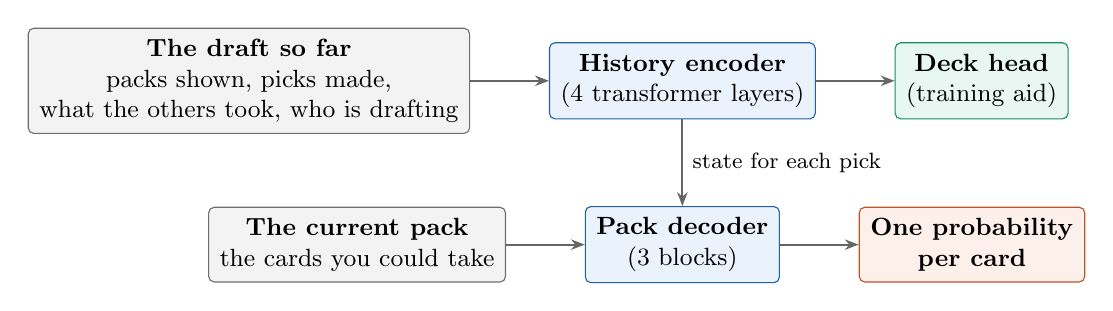
\begin{tikzpicture}[font=\small,node distance=0.55cm]
\node[box] (data) {\textbf{The draft so far}\\packs shown, picks made,\\what the others took, who is drafting};
\node[box=cblue,right=1.0cm of data] (hist) {\textbf{History encoder}\\(4 transformer layers)};
\node[box=cblue,below=1.1cm of hist] (dec) {\textbf{Pack decoder}\\(3 blocks)};
\node[box,left=1.0cm of dec] (pack) {\textbf{The current pack}\\the cards you could take};
\node[box=corange,right=1.0cm of dec] (out) {\textbf{One probability}\\\textbf{per card}};
\node[box=caqua,right=1.0cm of hist] (deck) {\textbf{Deck head}\\(training aid)};
\draw[arr] (data) -- (hist);
\draw[arr] (hist) -- node[right,font=\footnotesize]{state for each pick} (dec);
\draw[arr] (pack) -- (dec);
\draw[arr] (dec) -- (out);
\draw[arr] (hist) -- (deck);
\end{tikzpicture}
\caption{The model at the coarsest level. The deck head is only used during training; it gives the
history encoder an extra thing to learn (which picks will make the deck).}
\label{fig:big}
\end{figure}

\noindent A useful way to think about it: the history encoder answers ``who am I as a drafter right now?''
and the pack decoder answers ``given that, which of these cards do I want, considering what else is in the
pack?''.

Figure~\ref{fig:full} (page~\pageref{fig:full}) is the same model with nothing left out: every layer that has
trained weights, how many weights each one has, and the shape of every tensor for one draft. \textbf{Blue}
boxes have trained weights; the small blue number is how many. \textbf{Grey} boxes are data, \textbf{white}
boxes are fixed operations with no weights, $\oplus$ adds vectors, and {\color{corange}$\blacklozenge$} marks a
lookup in the card table. Shapes are per draft (a batch adds a leading $B$). The history-encoder layer is
stacked 4 times and the pack-decoder block 3 times, each copy with its own weights; the thin grey lines that
skip around each attention and MLP are the residual connections. Every decoder block reads the same history
states $\mathbf h$. Dropout (0.05) after each attention and MLP is not drawn. With the 65,792-weight pool layer
that only the no-history ablation uses, the counts add up to 8,357,889. The rest of this guide walks through
the figure from top to bottom, so it's worth keeping that page open while reading.

\begin{figure}[p]
\centering
\resizebox{!}{0.94\textheight}{% Every learned layer of PickNet for one draft (all_d256_ep2). \input by architecture.tex.
{\def\fT{\fontsize{5}{6}\selectfont}\def\fS{\fontsize{7}{8}\selectfont}\def\fF{\fontsize{8}{9.5}\selectfont}
\def\fN{\fontsize{10}{12}\selectfont}\def\fL{\fontsize{12}{14}\selectfont}
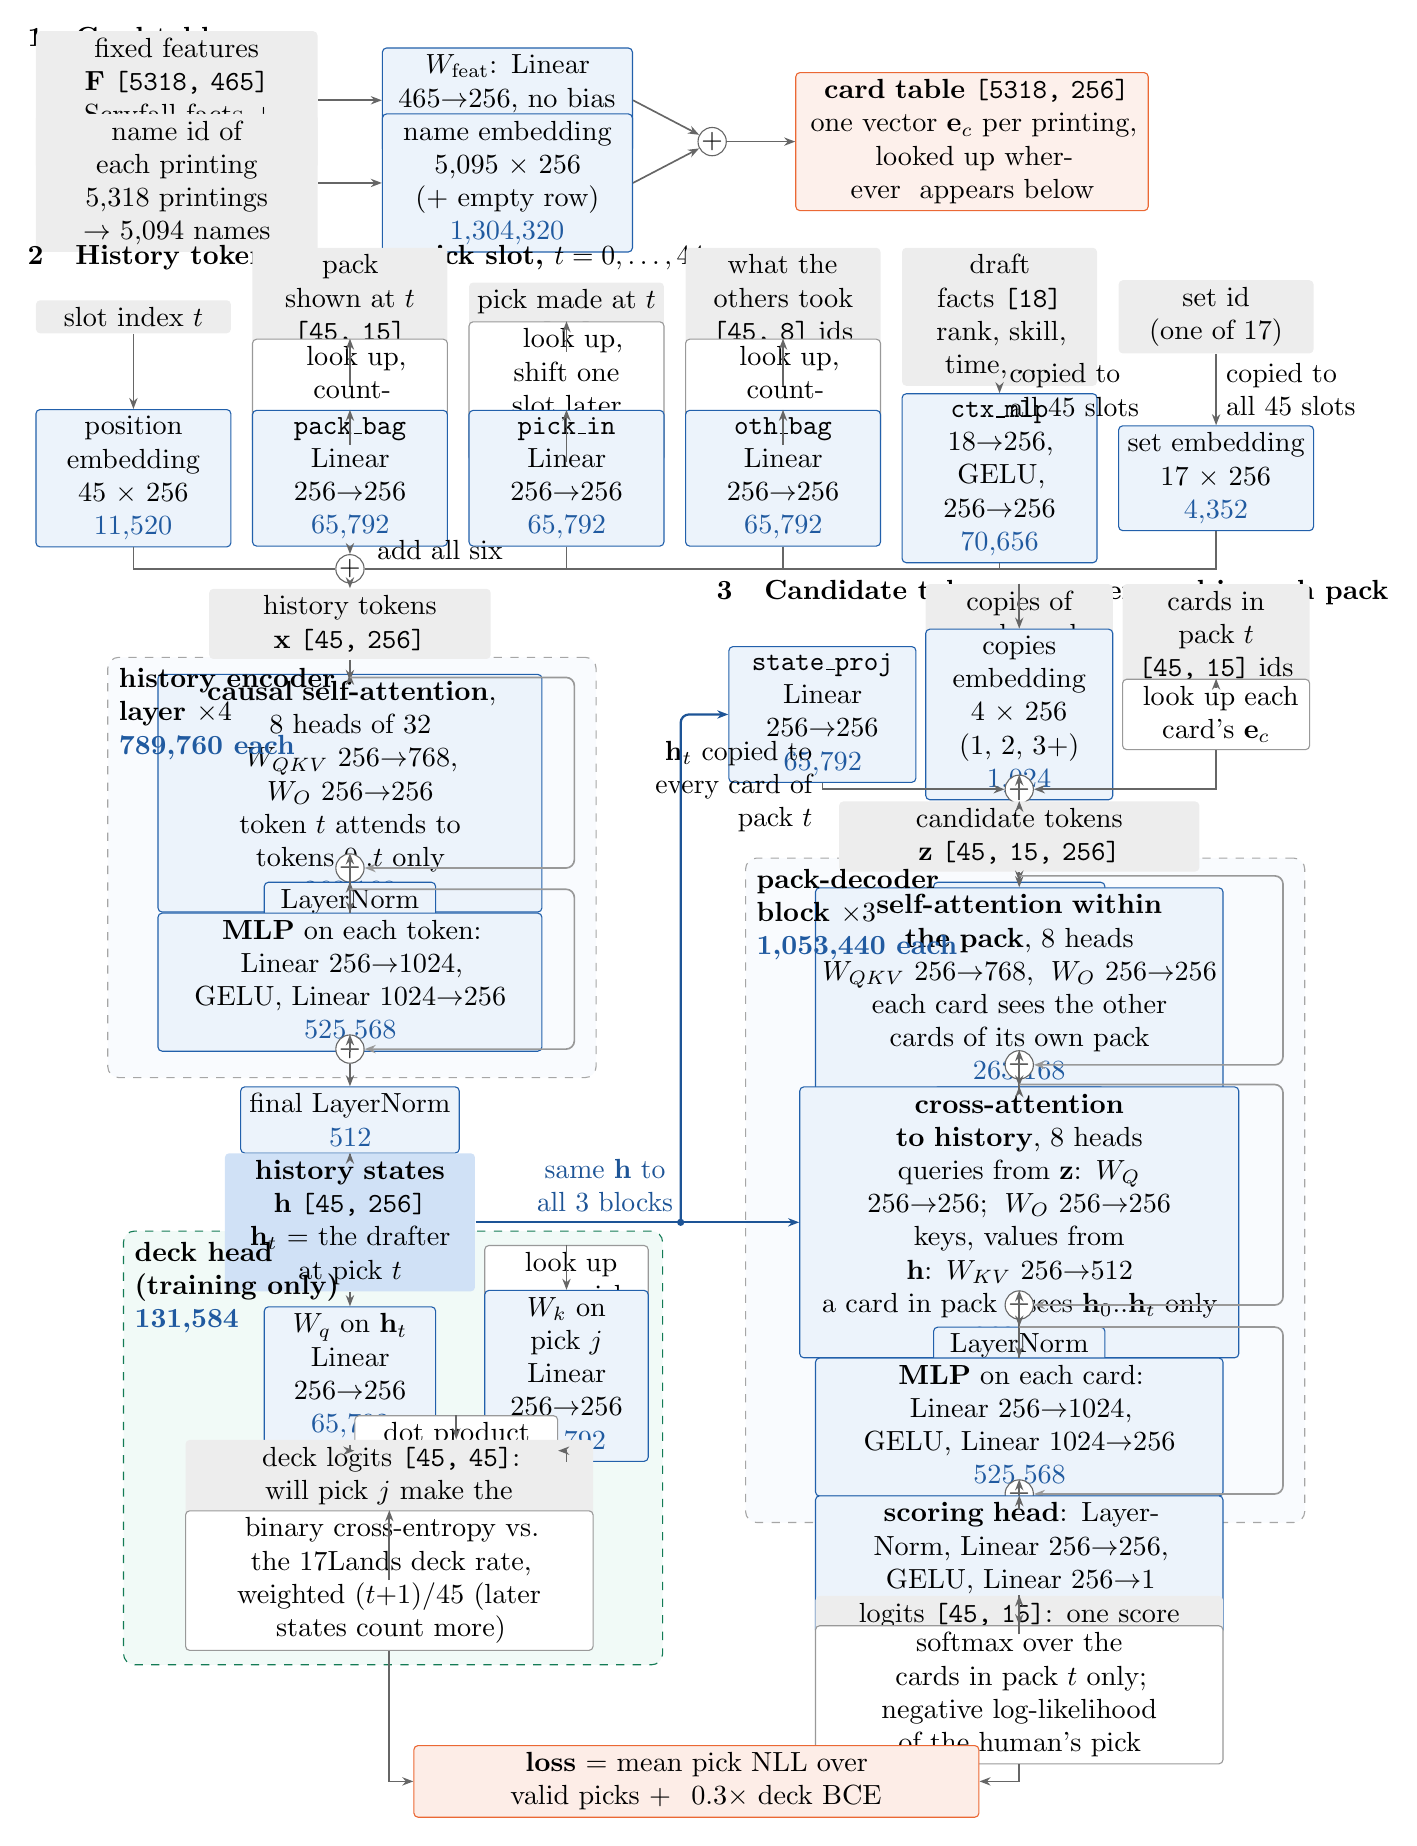
\begin{tikzpicture}[
  font=\fS,
  L/.style={draw=cblue!80!black,fill=cblue!9,rounded corners=1.5pt,align=center,inner sep=2.5pt,text width=#1},
  L/.default=2.3cm,
  O/.style={draw=black!40,fill=white,rounded corners=1.5pt,align=center,inner sep=2.5pt,text width=#1},
  O/.default=2.3cm,
  T/.style={fill=black!7,rounded corners=1.5pt,align=center,inner sep=2.5pt,text width=#1},
  T/.default=2.3cm,
  plus/.style={circle,draw=black!60,fill=white,inner sep=0pt,minimum size=3.4mm,font=\fF},
  a/.style={-{Stealth[length=4pt]},draw=black!60,semithick},
  ln/.style={draw=black!60,semithick},
  res/.style={-{Stealth[length=4pt]},draw=black!40,semithick,rounded corners=3pt},
  hb/.style={-{Stealth[length=4pt]},draw=cblue!70!black,thick,rounded corners=3pt},
  grp/.style={draw=black!35,dashed,rounded corners=4pt,inner sep=5pt},
  hd/.style={font=\fF\bfseries,anchor=west,inner sep=0pt},
  gl/.style={font=\fS\bfseries,anchor=north west,inner sep=0pt,align=left},
]
\def\pn#1{\\{\fT\color{cblue!75!black}#1}}
\def\shape#1{{\ttfamily[#1]}}
\def\lk{{\color{corange}$\blacklozenge$}}

% ------------------------------------------------------------ 1. card table
\node[hd] at (0,0) {1\quad Card table};
\node[T=3.4cm] (F) at (1.9,-0.8) {fixed features $\mathbf F$ \shape{5318, 465}\\Scryfall facts + rules-text embedding};
\node[L=3.0cm] (WF) at (6.1,-0.8) {$W_{\text{feat}}$: Linear 465$\to$256, no bias\pn{119,040}};
\node[T=3.4cm] (NID) at (1.9,-1.85) {name id of each printing\\5,318 printings $\to$ 5,094 names};
\node[L=3.0cm] (NE) at (6.1,-1.85) {name embedding\\5,095 $\times$ 256 (+ empty row)\pn{1,304,320}};
\node[plus] (pa) at (8.7,-1.325) {+};
\node[T=4.3cm,draw=corange,fill=corange!10] (TAB) at (12.0,-1.325)
  {\lk\ \textbf{card table} \shape{5318, 256}\\one vector $\mathbf e_c$ per printing,\\looked up wherever \lk\ appears below};
\draw[a] (F) -- (WF);
\draw[a] (NID) -- (NE);
\draw[a] (WF.east) -- (pa);
\draw[a] (NE.east) -- (pa);
\draw[a] (pa) -- (TAB);

% ------------------------------------------------------------ 2. history tokens
\node[hd] at (0,-2.8) {2\quad History tokens: one per pick slot, $t = 0,\dots,44$};
\foreach \k/\x in {1/1.35,2/4.1,3/6.85,4/9.6,5/12.35,6/15.1} \coordinate (c\k) at (\x,0);
\node[T] (i1) at (c1|-0,-3.55) {slot index $t$};
\node[T] (i2) at (c2|-0,-3.55) {pack shown at $t$\\\shape{45, 15} ids + copies};
\node[T] (i3) at (c3|-0,-3.55) {pick made at $t$\\\shape{45}};
\node[T] (i4) at (c4|-0,-3.55) {what the others took\\\shape{45, 8} ids + copies};
\node[T] (i5) at (c5|-0,-3.55) {draft facts \shape{18}\\rank, skill, time, \ldots};
\node[T] (i6) at (c6|-0,-3.55) {set id\\(one of 17)};
\node[O] (o2) at (c2|-0,-4.5) {\lk\ look up,\\count-weighted mean};
\node[O] (o3) at (c3|-0,-4.5) {\lk\ look up, shift one\\slot later (zero at $t{=}0$)};
\node[O] (o4) at (c4|-0,-4.5) {\lk\ look up,\\count-weighted mean};
\node[L] (l1) at (c1|-0,-5.6) {position embedding\\45 $\times$ 256\pn{11,520}};
\node[L] (l2) at (c2|-0,-5.6) {{\ttfamily pack\_bag}\\Linear 256$\to$256\pn{65,792}};
\node[L] (l3) at (c3|-0,-5.6) {{\ttfamily pick\_in}\\Linear 256$\to$256\pn{65,792}};
\node[L] (l4) at (c4|-0,-5.6) {{\ttfamily oth\_bag}\\Linear 256$\to$256\pn{65,792}};
\node[L] (l5) at (c5|-0,-5.6) {{\ttfamily ctx\_mlp}\\18$\to$256, GELU, 256$\to$256\pn{70,656}};
\node[L] (l6) at (c6|-0,-5.6) {set embedding\\17 $\times$ 256\pn{4,352}};
\draw[a] (i1) -- (l1);
\foreach \k in {2,3,4} {\draw[a] (i\k) -- (o\k); \draw[a] (o\k) -- (l\k);}
\draw[a] (i5) -- node[right,font=\fT,align=left]{copied to\\all 45 slots} (l5);
\draw[a] (i6) -- node[right,font=\fT,align=left]{copied to\\all 45 slots} (l6);
\node[plus] (pt) at (c2|-0,-6.75) {+};
\draw[a] (l2) -- (pt);
\draw[ln] (l1.south) |- (pt.west);
\draw[ln] (l6.south) |- (pt.east);
\foreach \k in {3,4,5} \draw[ln] (l\k.south) -- (l\k.south|-pt.center);
\node[font=\fT,above right=0pt and 1pt] at (pt.east) {add all six};

% ------------------------------------------------------------ 3. history encoder (left column)
\def\xc{4.1}
\node[T=3.4cm] (x) at (\xc,-7.45) {history tokens $\mathbf x$ \shape{45, 256}};
\draw[a] (pt) -- (x);
\node[L=2.0cm] (eln1) at (\xc,-8.6) {LayerNorm\pn{512}};
\node[L=4.7cm] (esa) at (\xc,-9.6) {\textbf{causal self-attention}, 8 heads of 32\\$W_{QKV}$ 256$\to$768,\; $W_O$ 256$\to$256\\token $t$ attends to tokens $0..t$ only\pn{263,168}};
\node[plus] (ep1) at (\xc,-10.55) {+};
\node[L=2.0cm] (eln2) at (\xc,-11.15) {LayerNorm\pn{512}};
\node[L=4.7cm] (emlp) at (\xc,-12.0) {\textbf{MLP} on each token: Linear 256$\to$1024,\\GELU, Linear 1024$\to$256\pn{525,568}};
\node[plus] (ep2) at (\xc,-12.85) {+};
\draw[a] (x) -- (eln1); \draw[a] (eln1) -- (esa); \draw[a] (esa) -- (ep1);
\draw[a] (ep1) -- (eln2); \draw[a] (eln2) -- (emlp); \draw[a] (emlp) -- (ep2);
\draw[res] (\xc,-8.13) -| (6.95,-9.0) |- (ep1.east);
\draw[res] (\xc,-10.82) -| (6.95,-11.5) |- (ep2.east);
\begin{scope}[on background layer]
\node[grp,fill=cblue!3,fit={(eln1)(esa)(emlp)(ep2)(7.05,-8.05)(1.2,-8.1)}] (enc) {};
\end{scope}
\node[gl] at ([shift={(4pt,-4pt)}]enc.north west) {history encoder\\layer {\fN$\times 4$}\\\textcolor{cblue!75!black}{\fT 789,760 each}};
\node[L=2.6cm] (fln) at (\xc,-13.75) {final LayerNorm\pn{512}};
\draw[a] (ep2) -- (fln);
\node[T=3.0cm,fill=cblue!22] (h) at (\xc,-15.05) {\textbf{history states} $\mathbf h$ \shape{45, 256}\\$\mathbf h_t$ = the drafter at pick $t$};
\draw[a] (fln) -- (h);

% ------------------------------------------------------------ 4. candidate tokens (right column)
\def\xr{12.6}
\node[hd] at (8.75,-7.05) {3\quad Candidate tokens: one per card in each pack};
\node[T=2.2cm] (ccnt) at (\xr,-7.6) {copies of each card\\\shape{45, 15}};
\node[T=2.2cm] (cidx) at (15.1,-7.6) {cards in pack $t$\\\shape{45, 15} ids};
\node[L=2.2cm] (sp) at (10.1,-8.6) {{\ttfamily state\_proj}\\Linear 256$\to$256\pn{65,792}};
\node[L=2.2cm] (cp) at (\xr,-8.6) {copies embedding\\4 $\times$ 256 (1, 2, 3+)\pn{1,024}};
\node[O=2.2cm] (clk) at (15.1,-8.6) {\lk\ look up each card's $\mathbf e_c$};
\draw[a] (ccnt) -- (cp); \draw[a] (cidx) -- (clk);
\node[plus] (pc) at (\xr,-9.55) {+};
\draw[a] (sp) |- node[pos=0.3,left,font=\fT,align=right]{$\mathbf h_t$ copied to\\every card of\\pack $t$} (pc.west); \draw[a] (cp) -- (pc); \draw[a] (clk) |- (pc.east);
\node[T=4.4cm] (z) at (\xr,-10.15) {candidate tokens $\mathbf z$ \shape{45, 15, 256}};
\draw[a] (pc) -- (z);

% ------------------------------------------------------------ 5. deck head (left column, training only)
\node[O=1.9cm] (dpk) at (6.85,-16.0) {\lk\ look up every pick \shape{45, 256}};
\node[L=2.0cm] (wq) at (\xc,-17.0) {$W_q$ on $\mathbf h_t$\\Linear 256$\to$256\pn{65,792}};
\node[L=1.9cm] (wk) at (6.85,-17.0) {$W_k$ on pick $j$\\Linear 256$\to$256\pn{65,792}};
\node[O=2.4cm] (dot) at (5.45,-17.95) {dot product $\div\sqrt{256}$};
\node[T=5.0cm] (dl) at (4.6,-18.7) {deck logits \shape{45, 45}: will pick $j$ make the\\main deck? (scored for $j < t$ only)};
\node[O=5.0cm] (bce) at (4.6,-19.6) {binary cross-entropy vs.\ the 17Lands deck rate,\\weighted $(t{+}1)/45$ (later states count more)};
\draw[a] (h) -- (wq);
\draw[a] (dpk) -- (wk);
\draw[a] (wq) |- (dot); \draw[a] (wk) |- (dot);
\draw[a] (dot) -- (dot|-dl.north); \draw[a] (dl) -- (bce);
\begin{scope}[on background layer]
\node[grp,fill=caqua!6,draw=caqua!70!black,fit={(dpk)(wq)(wk)(dot)(dl)(bce)(1.4,-15.7)}] (deck) {};
\end{scope}
\node[gl,anchor=north west] at ([shift={(4pt,-4pt)}]deck.north west) {deck head\\(training only)\\\textcolor{cblue!75!black}{\fT 131,584}};

% ------------------------------------------------------------ 5. pack decoder (right column)
\node[L=2.0cm] (dln1) at (\xr,-11.15) {LayerNorm\pn{512}};
\node[L=5.0cm] (dsa) at (\xr,-12.1) {\textbf{self-attention within the pack}, 8 heads\\$W_{QKV}$ 256$\to$768,\; $W_O$ 256$\to$256\\each card sees the other cards of its own pack\pn{263,168}};
\node[plus] (dp1) at (\xr,-13.05) {+};
\node[L=2.0cm] (dln2) at (\xr,-13.75) {LayerNorm\pn{512}};
\node[L=5.4cm] (dca) at (\xr,-15.05) {\textbf{cross-attention to history}, 8 heads\\queries from $\mathbf z$: $W_Q$ 256$\to$256;\; $W_O$ 256$\to$256\\keys, values from $\mathbf h$: $W_{KV}$ 256$\to$512\\a card in pack $t$ sees $\mathbf h_0..\mathbf h_t$ only\pn{263,168}};
\node[plus] (dp2) at (\xr,-16.1) {+};
\node[L=2.0cm] (dln3) at (\xr,-16.8) {LayerNorm\pn{512}};
\node[L=5.0cm] (dmlp) at (\xr,-17.65) {\textbf{MLP} on each card: Linear 256$\to$1024,\\GELU, Linear 1024$\to$256\pn{525,568}};
\node[plus] (dp3) at (\xr,-18.5) {+};
\draw[a] (z) -- (dln1); \draw[a] (dln1) -- (dsa); \draw[a] (dsa) -- (dp1);
\draw[a] (dp1) -- (dln2); \draw[a] (dln2) -- (dca); \draw[a] (dca) -- (dp2);
\draw[a] (dp2) -- (dln3); \draw[a] (dln3) -- (dmlp); \draw[a] (dmlp) -- (dp3);
\draw[res] (\xr,-10.65) -| (15.95,-11.5) |- (dp1.east);
\draw[res] (\xr,-13.3) -| (15.95,-14.0) |- (dp2.east);
\draw[res] (\xr,-16.38) -| (15.95,-17.1) |- (dp3.east);
\begin{scope}[on background layer]
\node[grp,fill=cblue!3,fit={(dln1)(dsa)(dca)(dmlp)(dp3)(16.05,-10.6)(9.3,-11)}] (dec) {};
\end{scope}
\node[gl] at ([shift={(4pt,-4pt)}]dec.north west) {pack-decoder\\block {\fN$\times 3$}\\\textcolor{cblue!75!black}{\fT 1,053,440 each}};

% the history states feed state_proj and every decoder block's cross-attention
\draw[hb] (h.east) -- node[above,font=\fT,text=cblue!70!black,pos=0.4,align=center]{same $\mathbf h$ to\\all 3 blocks} (dca.west);
\draw[hb] (8.3,-15.05) -- (8.3,-8.6) -- (sp.west);
\fill[cblue!70!black] (8.3,-15.05) circle (1.3pt);

% ------------------------------------------------------------ 6. scoring + loss
\node[L=5.0cm] (head) at (\xr,-19.4) {\textbf{scoring head}: LayerNorm, Linear 256$\to$256,\\GELU, Linear 256$\to$1\pn{66,561}};
\node[T=5.0cm] (lg) at (\xr,-20.25) {logits \shape{45, 15}: one score per card in each pack};
\node[O=5.0cm] (sm) at (\xr,-21.05) {softmax over the cards in pack $t$ only;\\negative log-likelihood of the human's pick};
\draw[a] (dp3) -- (head); \draw[a] (head) -- (lg); \draw[a] (lg) -- (sm);
\node[T=7.0cm,fill=corange!12,draw=corange] (loss) at (8.5,-22.15) {\textbf{loss} = mean pick NLL over valid picks $+\;0.3\times$ deck BCE};
\draw[a] (sm) |- (loss.east);
\draw[a] (bce) |- (loss.west);
\end{tikzpicture}}
}
\caption{Every learned layer of PickNet, for one draft. Blue: trained weights (with counts). Grey: data.
White: fixed operations. {\color{corange}$\blacklozenge$}: card-table lookup.}
\label{fig:full}
\end{figure}

% =====================================================================
\section{What one training example looks like}\label{sec:data}

One training example is one \emph{whole draft} by one drafter, not one pick. Every draft is laid out on a
fixed grid of 3 packs $\times$ 15 pick slots $=$ \textbf{45 slots}, numbered $t=0,\dots,44$. Sets with 14- or
13-card packs leave the last one or two slots of each pack empty; those slots are masked out (ignored) in
the loss and in every metric.


For each slot $t$ the data holds:

\begin{center}
\footnotesize
\begin{tabular}{>{\raggedright}p{2.3cm}>{\raggedright}p{2.1cm}p{9.2cm}}
\toprule
name in code & shape per draft & meaning \\
\midrule
\code{idx}, \code{cnt} & \shape{45, 15} & the pack shown at $t$: up to 15 distinct card ids, and how many copies of each \\
\code{pick} & \shape{45} & the card the human took at $t$ \\
\code{target} & \shape{45} & which of the 15 \code{idx} slots that card is in (the answer) \\
\code{oidx}, \code{ocnt} & \shape{45, 8} & the cards the other seven drafters took from the pack that just came back (empty for the first 8 picks of each pack) \\
\code{ctx} & \shape{18} & facts about the draft, the same for all 45 slots (Section~\ref{sec:ctx}) \\
\code{sid} & scalar & which of the 17 sets this is \\
\code{valid} & \shape{45} & false for empty slots, so they don't count \\
\code{rate} & \shape{45} & training-only: how often each pick ended up in the main deck \\
\bottomrule
\end{tabular}
\end{center}

\begin{figure}[!htbp]
\centering
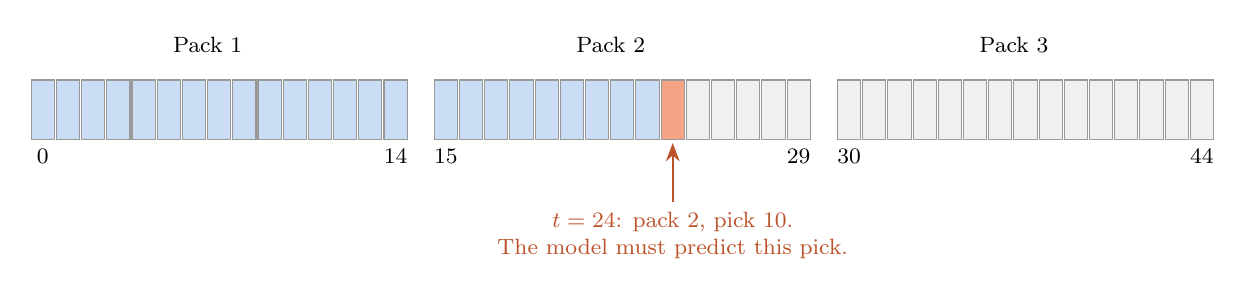
\begin{tikzpicture}[font=\scriptsize,x=0.32cm,y=0.5cm]
\foreach \k/\lab in {0/Pack 1,1/Pack 2,2/Pack 3} {
  \node[font=\footnotesize] at (\k*16+7,2.4) {\lab};
  \foreach \i in {0,...,14} {
    \pgfmathtruncatemacro{\t}{\k*15+\i}
    \ifnum\t<24
      \fill[cblue!25] (\k*16+\i,0) rectangle ++(0.92,1.5);
    \else\ifnum\t=24
      \fill[corange!60] (\k*16+\i,0) rectangle ++(0.92,1.5);
    \else
      \fill[black!6] (\k*16+\i,0) rectangle ++(0.92,1.5);
    \fi\fi
    \draw[black!40] (\k*16+\i,0) rectangle ++(0.92,1.5);
  }
}
\node[font=\footnotesize] at (0.46,-0.45) {0};
\node[font=\footnotesize] at (14.46,-0.45) {14};
\node[font=\footnotesize] at (16.46,-0.45) {15};
\node[font=\footnotesize] at (30.46,-0.45) {29};
\node[font=\footnotesize] at (32.46,-0.45) {30};
\node[font=\footnotesize] at (46.46,-0.45) {44};
\draw[corange!80!black,thick,-{Stealth}] (25.46,-1.6) node[below,align=center,font=\footnotesize]
  {$t=24$: pack 2, pick 10.\\The model must predict this pick.} -- (25.46,-0.1);
\end{tikzpicture}
\caption{The 45 slots of one draft. When predicting pick $t=24$ (orange), the drafter has seen every pack
up to and including this one, and has made every pick \emph{before} it (blue). Slots after it (grey) are
the future and must be hidden.}
\label{fig:grid}
\end{figure}

The model processes 32 drafts at a time (a \emph{batch}), so in the code most tensors have a leading
batch dimension $B=32$: \code{idx} is \shape{B, 45, 15}, and so on. Below we usually drop $B$ and talk
about one draft.

\paragraph{One forward pass predicts all 45 picks at once.} This is the single most important thing to
understand about how the model trains. The model does not run 45 separate times, once per pick. It reads
the whole draft in one go and outputs 45 sets of probabilities, one per slot. It can do this without
cheating because of the \emph{causal mask} (Section~\ref{sec:causal}): the computation for slot $t$ is
wired so that it can only use information from slots $\le t$ (packs) and $<t$ (picks). Feeding in the
real human picks as ``the picks made so far'' is called \emph{teacher forcing}; it is the same trick
language models use to predict every next word of a sentence in parallel.

% =====================================================================
\section{Step 1: turning a card into a vector}\label{sec:cards}

Neural networks work on lists of numbers, so the first job is to give every card a vector of $d=256$
numbers. Think of these as coordinates in a ``card space'' where similar cards land near each other. A card's
vector is the sum of two parts:

\begin{enumerate}
\item \textbf{A learned vector for the card's name.} A lookup table with one row of 256 numbers per
card name (5,094 names). The numbers start random and are tuned during training. Nothing tells the model
what they mean; it discovers that, say, one direction in the space means ``red'' and another means
``good in aggressive decks'' because that helps it predict picks. Reprints and basic lands share one row
across sets, because they are the same card.
\item \textbf{A projection of fixed card features.} Each printing (5,317 in all) also has a fixed list
of 465 numbers computed from Scryfall: colours, rarity, mana value, card types, power and toughness,
keywords, mana production, rules-text roles, and a 384-number text embedding of the rules text (from the
small language model \code{bge-small-en-v1.5}, with the card's own name blanked out). A learned
$465\times256$ matrix maps these into the same 256-dimensional space.
\end{enumerate}

\[
\mathbf{e}_c \;=\; \underbrace{\text{NameEmbedding}[\text{name}(c)]}_{\text{learned, per name}}
\;+\; \underbrace{W_{\text{feat}}\,\mathbf{f}_c}_{\text{learned map of fixed features}}
\qquad \mathbf{e}_c \in \mathbb{R}^{256}
\]

The features help most when a card has little data, and they give the name vector a sensible starting
point. The name vector is where the model stores what the features can't say, chiefly how strong the card
actually is in its format. The whole table, \shape{5318, 256} (one extra all-zero row for ``no card''), is
computed once per forward pass and then looked up everywhere a card appears. In the code this is
\code{CardTable}.

\paragraph{A ``bag'' of cards.} Several inputs are a set of cards rather than one card: the pack, the
cards the others took. The model turns a set into one vector by taking the \emph{count-weighted average}
of the card vectors, and then passing it through a learned $256\times256$ linear layer. This is what the
code calls \code{bag()}. A pack with two copies of card A and one of card B becomes
$\tfrac{2}{3}\mathbf{e}_A + \tfrac{1}{3}\mathbf{e}_B$. Averaging throws away order and exact
composition, but it keeps the gist: ``this pack is mostly green, with one strong rare''.

% =====================================================================
\section{Step 2: building one history token per pick}\label{sec:tokens}

The history encoder reads a sequence of 45 \emph{tokens}, one per pick slot. A token is just a vector of
256 numbers. Token $t$ is the \emph{sum} of six pieces of information, each first mapped into the same
256-number space:

\begin{figure}[!htbp]
\centering
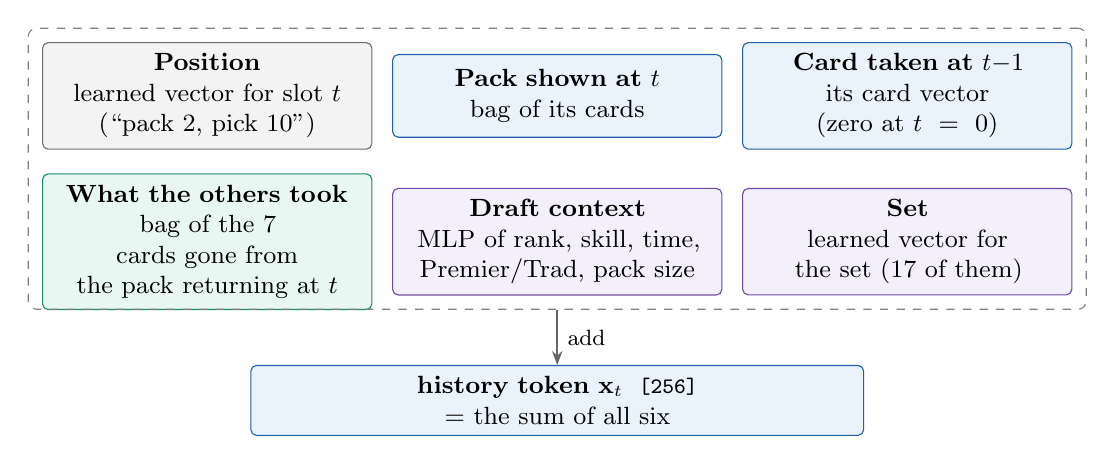
\begin{tikzpicture}[font=\small,
  part/.style={box=#1,text width=3.9cm,minimum height=1.05cm},
  part/.default=cgray]
\node[part] (p1) {\textbf{Position}\\learned vector for slot $t$\\(``pack 2, pick 10'')};
\node[part=cblue,right=0.25cm of p1] (p2) {\textbf{Pack shown at $t$}\\bag of its cards};
\node[part=cblue,right=0.25cm of p2] (p3) {\textbf{Card taken at $t{-}1$}\\its card vector\\(zero at $t=0$)};
\node[part=caqua,below=0.3cm of p1] (p4) {\textbf{What the others took}\\bag of the 7 cards gone from\\the pack returning at $t$};
\node[part=cpurple,right=0.25cm of p4] (p5) {\textbf{Draft context}\\MLP of rank, skill, time,\\Premier/Trad, pack size};
\node[part=cpurple,right=0.25cm of p5] (p6) {\textbf{Set}\\learned vector for\\the set (17 of them)};
\node[draw=black!50,dashed,rounded corners=3pt,inner sep=5pt,fit=(p1)(p6)] (all) {};
\node[box=cblue,below=0.7cm of all,text width=7.5cm] (tok) {\textbf{history token} $\mathbf{x}_t$ \;\shape{256}\\= the sum of all six};
\draw[arr] (all) -- node[right,font=\footnotesize]{add} (tok);
\end{tikzpicture}
\caption{The six ingredients of history token $t$. Each is mapped to 256 numbers and they are simply
added. Adding (rather than concatenating) is standard in transformers: the network learns to keep the
ingredients in roughly separate directions of the 256-dimensional space.}
\label{fig:token}
\end{figure}

\begin{itemize}
\item \textbf{Position.} One learned vector per slot (45 of them). Without it the model would not know
whether a token is pick 1 or pick 14, and the same pack means very different things at those two times.
\item \textbf{Pack shown at $t$.} The bag of the cards in the pack in front of the drafter now. Note the
asymmetry: token $t$ includes \emph{pack $t$} but only \emph{pick $t-1$}. The pick at $t$ is what we're
trying to predict, so it can't be an input to its own token. (Pick $t$ shows up one token later.)
\item \textbf{Card taken at $t-1$.} The vector of the card the drafter took last pick. Summed over all
earlier tokens by the attention layers, this is how the model knows the drafter's pool.
\item \textbf{What the others took.} Explained below; this is the input that lets the model read signals.
\item \textbf{Draft context.} Section~\ref{sec:ctx}.
\item \textbf{Set.} A learned vector per set, so the same model can behave differently in different
formats (a 3-mana 2/3 is great in one set and filler in another).
\end{itemize}

\subsection{``What the others took''}

With eight drafters, a pack you see at pick $p$ comes back to you at pick $p+8$, after each of the other
seven has taken one card from it. Comparing the two snapshots tells you exactly which seven cards the
table took, even though the data never says who the other drafters are.

\begin{figure}[!htbp]
\centering
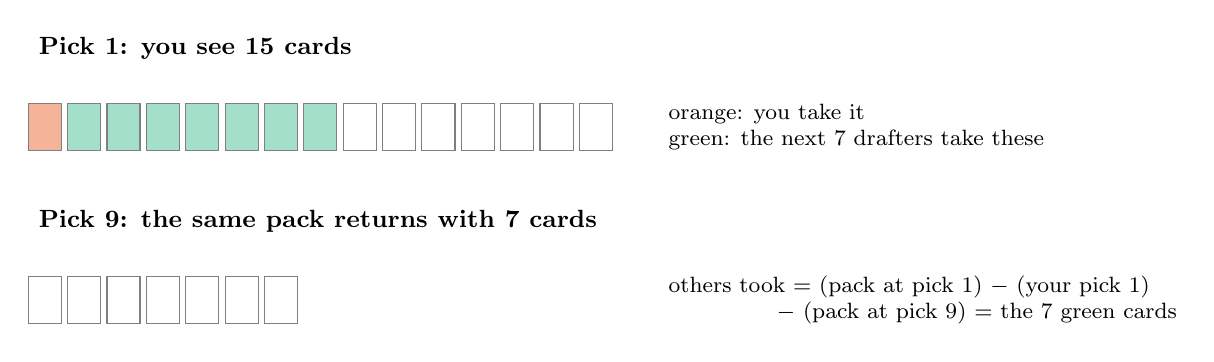
\begin{tikzpicture}[font=\small,
  c/.style={draw=black!50,fill=#1,minimum width=0.42cm,minimum height=0.6cm,inner sep=0pt},
  c/.default=white]
\node[anchor=west,font=\small\bfseries] at (-0.2,1.0) {Pick 1: you see 15 cards};
\foreach \i in {0,...,14} {
  \ifnum\i=0 \node[c=corange!50] at (\i*0.5,0) {}; \else
  \ifnum\i<8 \node[c=caqua!40] at (\i*0.5,0) {}; \else \node[c] at (\i*0.5,0) {}; \fi\fi
}
\node[anchor=west,font=\footnotesize,align=left] at (7.8,0) {orange: you take it\\green: the next 7 drafters take these};
\node[anchor=west,font=\small\bfseries] at (-0.2,-1.2) {Pick 9: the same pack returns with 7 cards};
\foreach \i in {8,...,14} \node[c] at (\i*0.5-4,-2.2) {};
\node[anchor=west,font=\footnotesize,align=left] at (7.8,-2.2)
  {others took $=$ (pack at pick 1) $-$ (your pick 1)\\\hspace{4.6em}$-$ (pack at pick 9) $=$ the 7 green cards};
\end{tikzpicture}
\caption{How ``what the others took'' is computed (\code{others\_taken()} in the code). The same
subtraction works for every pick from 9 onward in each pack; for picks 1--8 nothing has come back yet, so
this input is zero.}
\label{fig:others}
\end{figure}

Why it matters: if the green cards you passed are all gone but the blue ones wheel, blue is probably open.
Humans call this reading signals. The ablation in the paper finds the whole history (this input plus the
attention over earlier packs) adds about 1 point of accuracy, mostly in pack 3.

\subsection{Draft context}\label{sec:ctx}

Eighteen numbers describe the draft as a whole and are identical for all 45 tokens:

\begin{center}\small
\begin{tabular}{lcl}
\toprule
feature & numbers & encoding \\
\midrule
rank & 7 & one-hot: bronze, silver, gold, platinum, diamond, mythic, unknown \\
17Lands win rate & 2 & centred and scaled, plus a ``missing'' flag \\
17Lands games played & 2 & $\log_{10}$ of games, plus a ``missing'' flag \\
days since the format opened & 2 & linear and log-scaled \\
calendar time & 1 & years since 2023 \\
Traditional draft & 1 & 1 for Traditional (best-of-three), 0 for Premier \\
pack size & 3 & one-hot: 13, 14 or 15 cards \\
\bottomrule
\end{tabular}
\end{center}

A small two-layer network (an MLP: $18\to256\to256$) turns them into a 256-number vector that is added to
every token. This is how the model knows Premier from Traditional, mythic from bronze, week 1 from
week 8. Time is a continuous number rather than a ``which week'' lookup because the test drafts come from
the end of each format, in weeks no training draft covers; a lookup would have nothing learned for them.

% =====================================================================
\section{Step 3: the history encoder}\label{sec:causal}

Now we have 45 tokens, but each one only knows about its own slot. Token 24 holds pack 24 and pick 23, but
not pick 5. The history encoder's job is to let every token gather information from the earlier ones, so
that the output at slot $t$ summarises the \emph{whole} draft up to $t$. It does this with
\emph{self-attention}.

\subsection{Attention in one paragraph}

Each token computes three vectors from itself: a \emph{query} (``what am I looking for?''), a \emph{key}
(``what do I contain?'') and a \emph{value} (``what do I pass on if you pick me?''). Token $t$ compares its
query with every other token's key; the better the match, the bigger the weight. It then takes the
weighted average of the values and adds it to itself. So token 24 might learn to look hard at the tokens
where the drafter took red cards, and pull in ``I am red'' from them. The query, key and value maps are
learned. PickNet uses 8 \emph{heads}: 8 independent attention patterns run side by side, each on a 32-number
slice of the vector, so one head can track colours while another tracks the curve.

A transformer \emph{layer} is one attention step followed by a small per-token MLP ($256\to1024\to256$),
each wrapped with layer normalisation and a residual (``add the result back to the input'') connection.
The history encoder stacks \textbf{4} of these layers, so information can be gathered and recombined four
times.

\subsection{The causal mask}

If token 24 could attend to token 30, it would see pick 29, which is in the future. The \emph{causal
mask} forbids that: token $t$ may attend only to tokens $0,\dots,t$.

\begin{figure}[!htbp]
\centering
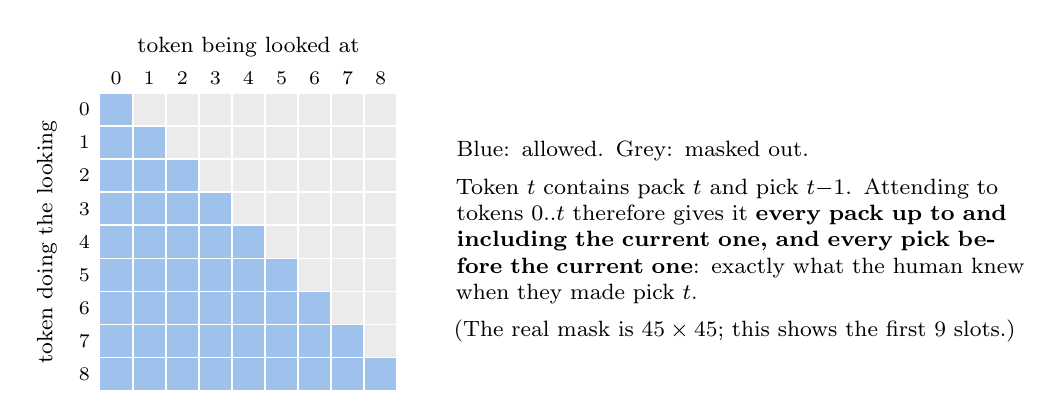
\begin{tikzpicture}[x=0.42cm,y=0.42cm,font=\scriptsize]
\foreach \r in {0,...,8} {
  \foreach \c in {0,...,8} {
    \ifnum\c>\r \fill[black!8] (\c,-\r) rectangle ++(1,-1);
    \else \fill[cblue!45] (\c,-\r) rectangle ++(1,-1); \fi
    \draw[white,line width=0.6pt] (\c,-\r) rectangle ++(1,-1);
  }
  \node[anchor=east] at (0,-\r-0.5) {\r};
  \node at (\r+0.5,0.45) {\r};
}
\node[font=\footnotesize,rotate=90] at (-1.6,-4.5) {token doing the looking};
\node[font=\footnotesize] at (4.5,1.4) {token being looked at};
\node[anchor=west,font=\footnotesize,align=left,text width=7.2cm] at (10.5,-4.5) {
  Blue: allowed. Grey: masked out.\\[4pt]
  Token $t$ contains pack $t$ and pick $t{-}1$. Attending to tokens $0..t$ therefore gives it
  \textbf{every pack up to and including the current one, and every pick before the current one}:
  exactly what the human knew when they made pick $t$.\\[4pt]
  (The real mask is $45\times45$; this shows the first 9 slots.)};
\end{tikzpicture}
\caption{The causal mask. Because of it, one pass over the whole draft gives 45 honest states, each
blind to its own pick and everything after.}
\label{fig:mask}
\end{figure}

The output is one \emph{state} $\mathbf{h}_t$ (256 numbers) per slot, after a final layer normalisation.
$\mathbf{h}_t$ is the model's summary of the drafter at the moment of pick $t$. Because of the mask, it is
the same whether you compute it by feeding the full draft or only the first $t+1$ slots; that is what makes
the parallel training of Section~\ref{sec:data} legitimate, and it is also how you use the model live:
feed in the draft so far, read off the last slot.

% =====================================================================
\section{Step 4: candidate tokens}

The history encoder knows the drafter; now the model must score the cards in pack $t$. Each card $c$ in
that pack gets its own \emph{candidate token}, again a sum:

\[
\mathbf{z}_{t,c} \;=\; \underbrace{\mathbf{e}_c}_{\text{card vector}}
\;+\; \underbrace{\text{CopiesEmbedding}[\text{copies}_c]}_{\text{1, 2 or 3+ copies in the pack}}
\;+\; \underbrace{W_{\text{state}}\,\mathbf{h}_t}_{\text{the drafter right now}}
\]

So the candidate ``Card A at pick 24'' starts out knowing both what Card A is and who is looking at it.
Every pack slot gets up to 15 candidates (fewer as the pack empties), so across the draft there are
$45\times15$ candidate tokens, \shape{45, 15, 256}. Empty candidate positions are masked out.

% =====================================================================
\section{Step 5: the pack decoder}

The pack decoder refines the candidate tokens with \textbf{3 blocks}. Each block does three things, each
with layer normalisation before it and a residual connection around it:

\begin{figure}[!htbp]
\centering
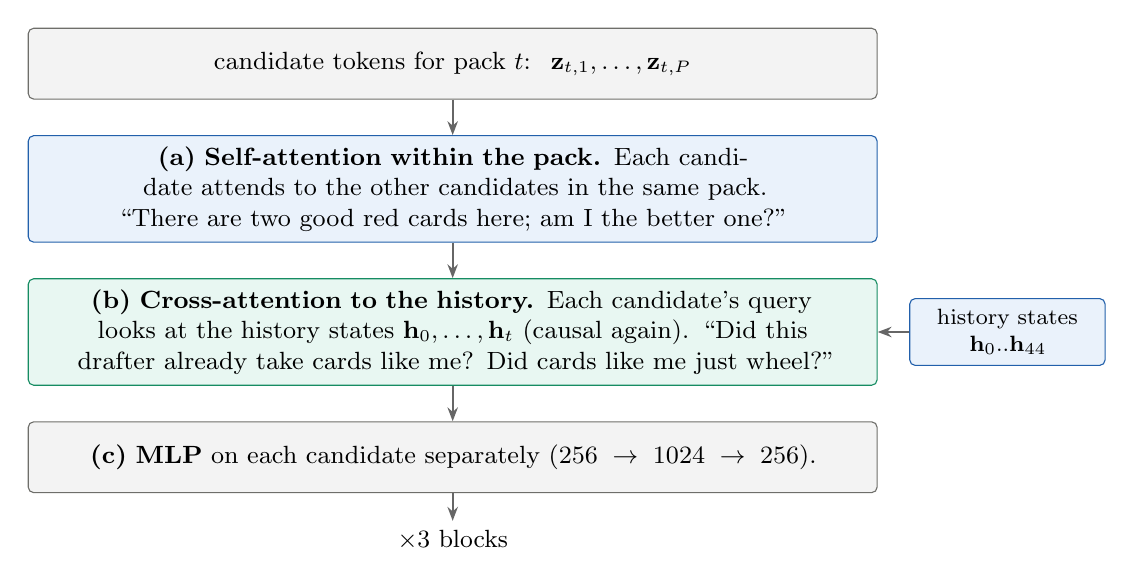
\begin{tikzpicture}[font=\small,node distance=0.45cm,
  st/.style={box=#1,text width=10.5cm,minimum height=0.9cm}]
\node[st=cgray] (in) {candidate tokens for pack $t$: \;$\mathbf{z}_{t,1},\dots,\mathbf{z}_{t,P}$};
\node[st=cblue,below=of in] (sa) {\textbf{(a) Self-attention within the pack.} Each candidate attends to
the other candidates in the same pack. ``There are two good red cards here; am I the better one?''};
\node[st=caqua,below=of sa] (ca) {\textbf{(b) Cross-attention to the history.} Each candidate's query
looks at the history states $\mathbf{h}_0,\dots,\mathbf{h}_t$ (causal again). ``Did this drafter already
take cards like me? Did cards like me just wheel?''};
\node[st=cgray,below=of ca] (mlp) {\textbf{(c) MLP} on each candidate separately ($256\to1024\to256$).};
\node[below=0.35cm of mlp,font=\small] (rep) {$\times 3$ blocks};
\draw[arr] (in) -- (sa);
\draw[arr] (sa) -- (ca);
\draw[arr] (ca) -- (mlp);
\draw[arr] (mlp) -- (rep);
\node[box=cblue,right=0.4cm of ca,text width=2.2cm,font=\footnotesize] (h) {history states\\$\mathbf{h}_0..\mathbf{h}_{44}$};
\draw[arr] (h) -- (ca);
\end{tikzpicture}
\caption{One pack-decoder block (\code{Block} in the code).}
\label{fig:block}
\end{figure}

\textbf{(a) is the step that matters most.} A pick-order bot scores each card on its own. But picking is
a \emph{comparison}: a decent red card is the right pick when it's the best card in the pack and the wrong
one next to a red bomb. Self-attention among the candidates lets each card's score depend on what it's
competing against. The paper's ablation credits this step with about 3 points of accuracy, three times
what the history of passed packs adds.

\textbf{(b) differs from what the history encoder did.} There, history tokens looked at other history
tokens. Here the \emph{candidates} ask the questions and the \emph{history states} answer. The candidate
for Card A at pick 24 can pull from any $\mathbf{h}_{s}$ with $s\le24$, so it can find, for instance, the
moment the drafter moved into a colour.

Self-attention here runs separately within each pack: the candidates of pick 24 never see the candidates
of pick 25. That's why the whole thing still fits in one parallel pass.

% =====================================================================
\section{Step 6: from scores to a pick}\label{sec:softmax}

After the last block, a small head (layer norm, $256\to256$, GELU, $256\to1$) turns each candidate token
into a single number, its \emph{logit} (score). The probability of taking card $c$ is the softmax over the
cards actually in the pack:

\[
P(\text{take } c \mid \text{everything so far}) \;=\;
\frac{\exp(\text{logit}_c)}{\sum_{c' \in \text{pack}_t} \exp(\text{logit}_{c'})}
\]

Cards not in the pack aren't candidates, so they get no probability at all. This ``softmax over only the
available options'' is the same as the conditional logit model economists use for consumer choice.

\paragraph{A worked example.} Suppose pack $t$ has five cards left and the model outputs these logits.
(The cards are made up for illustration.)

\begin{center}\small
\begin{tabular}{lcccc}
\toprule
card & logit & $\exp(\text{logit})$ & probability & \\
\midrule
A: on-colour removal spell & 2.1 & 8.17 & 0.574 & \textcolor{cblue}{\rule{2.87cm}{6pt}} \\
B: on-colour 2-drop & 1.3 & 3.67 & 0.258 & \textcolor{cblue}{\rule{1.29cm}{6pt}} \\
C: off-colour rare & 0.4 & 1.49 & 0.105 & \textcolor{cblue}{\rule{0.52cm}{6pt}} \\
D: on-colour filler & $-0.5$ & 0.61 & 0.043 & \textcolor{cblue}{\rule{0.21cm}{6pt}} \\
E: off-colour filler & $-1.2$ & 0.30 & 0.021 & \textcolor{cblue}{\rule{0.11cm}{6pt}} \\
\midrule
sum & & 14.24 & 1.000 & \\
\bottomrule
\end{tabular}
\end{center}

\begin{itemize}
\item \textbf{Top-1 accuracy}: the model's prediction is A. If the human took A, this pick counts as
correct. The paper's 70.8\% is the share of test picks where this happens.
\item \textbf{Loss (NLL)}: if the human took B, the loss for this pick is $-\ln 0.258 = 1.35$ nats; had
they taken A, it would be $-\ln 0.574 = 0.56$. Training lowers the average of this number over all valid
picks. Unlike top-1, it rewards being confidently right and punishes being confidently wrong, which is why
the paper reports both. The model averages 0.749 nats per pick on the test set.
\end{itemize}

Forced picks (the last card of a pack) have one candidate, so their probability is always 1 and their
loss 0. That's why the paper also reports accuracy on non-forced picks.

% =====================================================================
\section{The deck head: a training aid}

Alongside the pick loss, the model gets a second, smaller job, borrowed from the puder model: from the
state $\mathbf{h}_t$, predict for every earlier pick $j<t$ whether that card ends up in the drafter's main
deck.

\[
\text{deck logit}_{t,j} \;=\; \frac{(W_q\mathbf{h}_t)\cdot(W_k\mathbf{e}_{\text{pick}_j})}{\sqrt{256}}
\]

This is a dot product between ``the drafter at time $t$'' and ``the card picked at $j$''. The target is
the card's 17Lands main-deck rate for that drafter (a number between 0 and 1), scored with binary
cross-entropy. Later states get more weight (weight $(t+1)/45$), since by pack 3 the drafter's deck is
much clearer than at pick 2. This loss is multiplied by 0.3 and added to the pick loss.

\begin{figure}[!htbp]
\centering
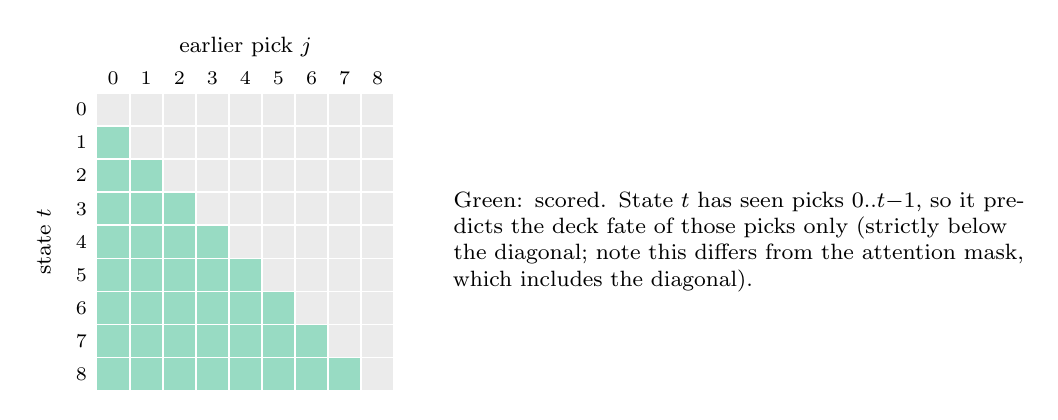
\begin{tikzpicture}[x=0.42cm,y=0.42cm,font=\scriptsize]
\foreach \r in {0,...,8} {
  \foreach \c in {0,...,8} {
    \ifnum\c<\r \fill[caqua!45] (\c,-\r) rectangle ++(1,-1);
    \else \fill[black!8] (\c,-\r) rectangle ++(1,-1); \fi
    \draw[white,line width=0.6pt] (\c,-\r) rectangle ++(1,-1);
  }
  \node[anchor=east] at (0,-\r-0.5) {\r};
  \node at (\r+0.5,0.45) {\r};
}
\node[font=\footnotesize,rotate=90] at (-1.6,-4.5) {state $t$};
\node[font=\footnotesize] at (4.5,1.4) {earlier pick $j$};
\node[anchor=west,font=\footnotesize,text width=7.2cm] at (10.5,-4.5) {
  Green: scored. State $t$ has seen picks $0..t{-}1$, so it predicts the deck fate of those picks only
  (strictly below the diagonal; note this differs from the attention mask, which includes the diagonal).};
\end{tikzpicture}
\caption{Which (state, pick) pairs the deck head is trained on.}
\end{figure}

Why bother? Knowing which of your picks will make the deck is close to knowing which archetype you are in,
and that is exactly what the history state needs to encode for good pick predictions. The extra target
pushes the history encoder toward that knowledge. The deck head is never used to make a pick, and the paper
notes it was not ablated, so how much it helps is unmeasured.

% =====================================================================
\section{Training}

\begin{itemize}
\item \textbf{Data.} 1.72M training drafts from 17 sets, Premier and Traditional, shuffled together. Each
batch is 32 drafts, so $32\times45 = 1{,}440$ picks contribute to each update (minus empty slots).
\item \textbf{Loss.} Mean pick NLL over valid picks $+\;0.3\times$ deck loss.
\item \textbf{Optimiser.} AdamW (weight decay 0.01), gradients clipped at norm 1, a one-cycle learning-rate
schedule: a short warm-up, then a cosine decay to near zero. One cycle is 53,791 steps, one pass over the
training drafts.
\item \textbf{Two epochs.} Epoch 1 peaks at learning rate $5\times10^{-4}$. Epoch 2 starts from epoch 1's
best weights, peaks at $2\times10^{-4}$ and sees the drafts in a new order.
\item \textbf{Early stopping.} Every 2,500 steps the model is scored on 4,000 held-out Premier drafts;
the best-scoring weights are kept.
\item \textbf{Regularisation.} Dropout 0.05 throughout. The ``pack dropout'' option (hide the packs from
the history for half the drafts) exists in the code but is off in the final model; it made no difference.
\end{itemize}

% =====================================================================
\section{Shapes and sizes}

Tensor shapes through one forward pass, for a batch of $B=32$ drafts ($T=45$ slots, $P=15$ candidate
positions, $d=256$):

\begin{center}\small
\begin{tabular}{lll}
\toprule
stage & shape & code \\
\midrule
card table & \shape{5318, 256} & \code{tab = self.cards()} \\
pack bag, pick vector, others bag, position & \shape{B, 45, 256} each & \code{bag(...)}, \code{prev}, \code{self.pos} \\
context, set & \shape{B, 1, 256}, broadcast to all 45 & \code{ctx\_mlp}, \code{set\_emb} \\
history tokens $\mathbf{x}$ & \shape{B, 45, 256} & \code{h} before \code{self.hist} \\
history states $\mathbf{h}$ & \shape{B, 45, 256} & \code{h} after \code{hist\_norm} \\
candidate tokens $\mathbf{z}$ & \shape{B, 45, 15, 256} & \code{x} \\
\quad (a) self-attention & over the 15 within each of $B\cdot45$ packs & \code{Block}, first half \\
\quad (b) cross-attention & $45\cdot15$ queries per draft over 45 states & \code{Block}, second half \\
logits & \shape{B, 45, 15} & \code{self.head(x)} \\
deck logits & \shape{B, 45, 45} & \code{deck\_logits()} \\
\bottomrule
\end{tabular}
\end{center}

Where the 8.36M parameters are:

\begin{center}\small
\begin{tabular}{lrr}
\toprule
component & parameters & share \\
\midrule
card table (5,094 name vectors + feature projection) & 1,423,360 & 17\% \\
history encoder (4 transformer layers + final norm) & 3,159,552 & 38\% \\
pack decoder (3 blocks) & 3,160,320 & 38\% \\
token input layers (pack, pick, others, context, position, set) & 283,904 & 3\% \\
candidate projection, copies, scoring head & 133,377 & 2\% \\
deck head & 131,584 & 2\% \\
unused (pool layer for the no-history ablation) & 65,792 & 1\% \\
\midrule
total & 8,357,889 & \\
\bottomrule
\end{tabular}
\end{center}

% =====================================================================
\section{Putting it together: one pick, start to finish}

Say we want the model's prediction for a mythic-rank Premier drafter at pack 2, pick 10 ($t=24$).

\begin{enumerate}
\item \textbf{Look up card vectors} for every card that appears anywhere in the draft so far.
\item \textbf{Build tokens 0--24.} Token 24 = position 24 + bag(the 6 cards in front of them) + vector of
the card they took at pick 9 of pack 2 + bag(the 7 cards the table took from this pack since they saw it at
pick 2) + context(mythic, Premier, day 23 of the format, \ldots) + the set's vector.
\item \textbf{Run the history encoder.} Four layers of causal attention. State $\mathbf{h}_{24}$ now
reflects all 24 earlier picks (their pool), every pack they saw, and every returning pack.
\item \textbf{Build 6 candidate tokens}, one per card in the pack: card vector + copies + projected
$\mathbf{h}_{24}$.
\item \textbf{Run the pack decoder.} In each of 3 blocks the six candidates compare themselves with each
other, consult $\mathbf{h}_0..\mathbf{h}_{24}$, and pass through an MLP.
\item \textbf{Score.} Six logits, a softmax over those six, and the highest-probability card is the
prediction.
\end{enumerate}

In training, steps 1--6 happen for all 45 slots and all 32 drafts in the batch at once, and the losses
from all valid picks are averaged before each update.

% =====================================================================
\section{FAQ}

\paragraph{Why not just feed the model ``the cards in my pool'' and ``the cards in the pack''?} That's
roughly the \emph{pool} baseline in the paper: a pick-order rating per card plus a learned card-by-pool
match score. It gets 64.4\% on MSH. Adding the within-pack comparison gets to 67.3\%, and the full history
to 68.2\%. The transformer machinery is what buys those points.

\paragraph{Does the model know who the other drafters are?} No. It only sees which cards vanished from
the packs that came back. It has to infer what the neighbours are drafting from that.

\paragraph{How does one model handle 17 sets?} Every set's cards live in one shared card table (reprints
share a vector), the set embedding tells the model which format it's in, and card features give new cards
a sensible starting point. Pooling the sets added 1.3 points over the best single-set model on MSH.

\paragraph{Does it know Premier from Traditional?} Yes, through the Traditional flag in the draft
context (Section~\ref{sec:ctx}). It trains on both but is validated and tested on Premier only.

\paragraph{Can it draft a set it has never seen?} Not well. The name vectors for new cards would be
untrained. A features-only variant (no name vectors) trained on 7 other sets scores 50.8\% on unseen MSH,
barely above a pick-order bot fitted on MSH itself.

\paragraph{Is it drafting \emph{well}?} It imitates 17Lands users, who are above average but not
optimal. A high top-1 means ``picks like these humans'', not ``picks the best card''.

\end{document}
